% !TeX root = ../thuthesis-caishiyu.tex

\chapter{数据恢复机制设计}
\label{chap:recovery}

本章节将从设计目标,设计思路以及正确性来介绍数据恢复的设计。
同时本章节介绍了对于 N2DB 存储引擎的修改以及代码层面的系统实现。

\section{设计目标}


数据库存储引擎的故障类型可以分为几种,事务故障,系统故障以及硬件故障。事务故障意味着事务执行的过程中出现了错误,通常通过数据库管理系统的回滚操作来清除掉。而系统故障通常包括操作系统故障以及宕机故障,通常会导致数据库管理系统运行中断。而硬件故障意味着存储介质出现严重错误,系统能难通过软件层面避免此问题。

数据恢复机制是数据库系统为了从系统故障中恢复成可工作状态而设计的。当系统中断时,DRAM 中的所有数据丢失,系统必须根据持久化介质上保存的数据将系统还原到系统中断时的状态。
传统的数据库通常使用日志系统记录所有的事务操作信息,在重启之后根据日志系统重做检查点之后的事务的操作,回滚未提交的事务的操作。

N2DB 使用 NVM 作为主要存储介质,大部分数据在系统故障后仍然保存在 NVM 上。
由于 N2DB 在运行过程中是无日志的,数据恢复缺乏了上一轮的运行信息。
数据恢复机制需要在无日志的前提下达到以下 3 个设计目标:

\textbf{重构页面分配信息:}N2DB 的主要数据均存储在 NVM 上,同时是按照页粒度分配且管理的。
然而分配器的分配是无日志的,因此 N2DB 需要在数据恢复阶段重构正确的页面分配信息。
系统在正确的分配信息的基础上才能回收已分配但未被使用的页面,进而防止内存泄漏问题。

\textbf{恢复数据结构:}系统需要在恢复服务之前得到所有数据结构的地址信息以及类型信息。
而页面分配信息仅能帮助系统得到页面的使用情况,而无法得到页面中所存储的数据结构信息。
因此 N2DB 需要将数据库的元数据持久化,并且提供一个固定的入口。
数据库的其他数据结构也需要妥善地设计。
系统才能根据元数据中的数据结构信息以及表格的模式信息获得所有表格中所有的记录数据。

\textbf{保证事务的原子性和持久化:}数据库管理系统在数据恢复的过程中需要遵循两个恢复原则:
保证提交事务的影响的持久化以及消除中止事务的影响。
由于 N2DB 在并发控制算法的设计中保证了当事务提交时,所有的数据均已持久化到 NVM 上。
因此数据恢复流程需要具有识别以及消除中止事务的影响的能力。

数据恢复只有在满足上述三个设计目标的前提下,才能确保系统在恢复后能够正确地提供服务。

\section{存储引擎的结构修改}

N2DB 为了在重启之后能够满足以上三个设计目标,需要对存储引擎进行重新设计,主要涉及两部分,分别是 NVM 分配器的结构修改以及数据库元信息区的结构设计。
修改后整体的存储引擎结构如图~\ref{fig:nvm-allocator} 所示。

\subsection{NVM 分配器的结构修改}。
从图~\ref{fig:nvm-allocator} 中可以看出,相对于之前的 NVM 分配器,新版的 NVM 分配器主要增加一个持久化指针数组。
该持久化指针数据存储于 NVM 文件的第二页,记录了数据库上所有数据结构的根指针。
通常而言,N2DB 的元数据的根指针会存放在持久化数组中的第一个位置。

\begin{figure}[ht]
    \centering
    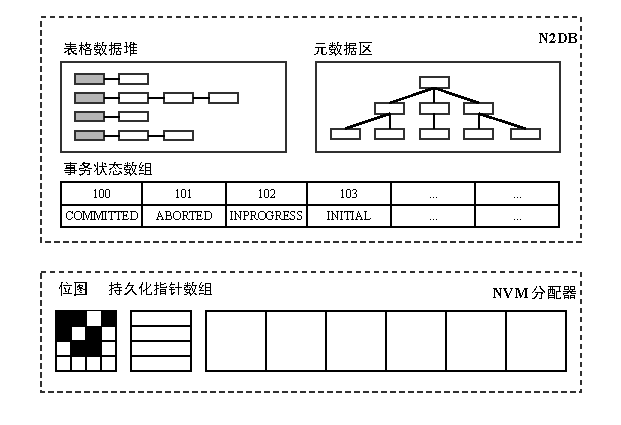
\includegraphics[width=1\linewidth]{figures/new-nvm-allocator}
    \caption{修改后的 N2DB 存储引擎的结构}
    \label{fig:nvm-allocator}
\end{figure}

\subsection{数据库元数据区的结构设计}

为了保证 N2DB 在故障恢复的过程中找到所有的数据库中所有的元数据, N2DB 需要增加一个元数据区负责存储和管理所有数据库的元信息。
元数据区的结构如图~\ref{fig:catalog} 所示。
元数据区中的数据结构组织成一颗三层高的树,其根节点的指针存储在 NVM 分配器的指针区域中。元数据区根据树的层次分别由三类数据结构,从根节点到叶节点分别是 N2DB 元数据,数据库元数据以及表格元数据。

\begin{figure}
    \centering
    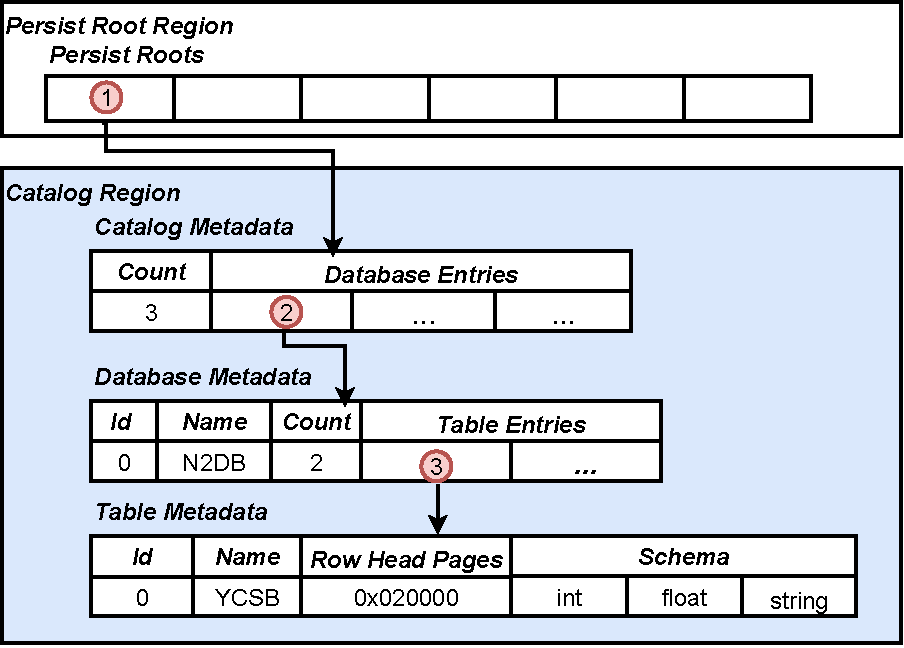
\includegraphics[width=1\linewidth]{figures/catalog.pdf}
    \caption{数据库元信息区的结构}
    \label{fig:catalog}
\end{figure}

N2DB 元数据中记录的整个存储引擎的元数据,比如存储引擎是否被初始化,这一轮的事务 ID 的起始值等信息。一个存储引擎可以创建多个数据库,因此 N2DB 元数据中还存放着数据库元数据的数量有以及各个数据库元数据的地址。

数据库元数据中存储这数据库的标识符,数据库的名称。同时数据库元数据中存储着一个定长的指针数组,其中的每个指针均是指向从属于该数据库的表格元数据。为了减少恢复时的开销,系统同样存储着表格数量。


表格元数据用于存储表格的所有元数据,包括表格的标识符等信息。同时表格元信息中也存储了模式信息,数据库管理系统可以借此计算出表格中所有的 head 和 version 的大小。在系统运行时,表格会将申请获得的页面的地址记录在表格元数据中。




\section{数据恢复机制设计思路}

根据上述三个设计目标,本文将 N2DB 的数据恢复流程分为三个阶段,分别是 NVM 分配器的恢复,数据库元数据的恢复以及记录数据的恢复。

\subsection{NVM 分配器的恢复}
\label{ssec:allocator-recovery}

NVM 分配器的恢复的目的在于回收所有未分配和分配但未被分配的页面。
当系统重启之后,N2DB 首先扫描 NVM 分配器的位图。
根据位图中的数据得到在系统宕机时的页面分配信息。
NVM 分配器将 bitmap 中所有状态为未分配的页面添加到一个空闲页面队列。

由于 NVM 分配器是无日志的分配的,因此位图中被标记位已分配的页面有可能没有任何数据结构使用该页面。
如果不回收此类页面则会造成内存泄漏。
然而根据 NVM 分配器自身的元数据无法回收分配但未被使用的页面。
此类页面会在后续步骤中由上层系统协助回收,具体的流程会在后续章节涉及到。

\subsection{数据库元数据的恢复}
\label{ssec:metadata-recovery}

数据库元数据的恢复的主要目的在于在 NVM 上找到所有数据库的数据结构,找到所有的记录相关的数据结构,重新设置数据库在重启之后的事务状态以及协助 NVM 分配器回收分配但未分配的空间。
数据库的元数据恢复的流程如下:

首先,N2DB 需要在 NVM 上找到所有元数据,并在内存中建立起数据库的索引。
目录是存储引擎中所有的数据库,表格以及列信息的索引。
N2DB 根据 NVM 分配器的接口得到 N2DB 元数据的地址。
由于 N2DB 上所有元数据组织成树状数据结构,N2DB 可以根据 N2DB 元数据中记录的信息,遍历地找到所有的数据库元数据以及表格元数据。
N2DB 在遍历树的过程中,需要根据持久化的元数据中的标记位信息来判断数据库或者表格是否创建成功。
如果数据库以及表格是创建失败的,N2DB 需要无视该数据库或表格的信息。
N2DB 将所有创建成功的数据库以及表格按照正确的层级关系添加到数据库目录中。
在此过程中,N2DB 需要统计所有创建成功的数据库和表格的元数据的空间使用情况。

其次,N2DB 根据表格的元数据中记录的 head 页面入口以及 version 页面入口得到所有表格的页面信息。
N2DB 根据表格元数据中的模式信息计算出各个表格的记录的 head 以及 version 的长度。
之后 N2DB 获得数据库中所有版本链的入口,以及表格中每个版本链所对应的行标识符。
在此过程中,N2DB 需要统计所有表格所管理的页面的使用情况。

接下来,N2DB 需要根据事务状态信息重新设置本轮运行的起始事务 ID。
事务状态数组中记录着上一轮活跃的事务 ID 的最大值以及最小值。
N2DB 根据事务状态数组中的数据更新本轮事务的起始 ID。
之后 N2DB 扫描事务状态数组中上一轮活跃的事务区间,将其中所有未结束的事务状态设置为 ABORTED。

最后,系统需要协助 NVM 分配器回收所有分配但未被使用的页面。
N2DB 在前几步记录了所有被数据库所使用的空间的信息。
之后 N2DB 将汇总后的空间使用情况传递给 NVM 分配器,NVM 分配器将会回收不被数据库使用的但状态为已分配的页面。



\subsection{记录数据的恢复}
\label{ssec:record-recovery}

当 N2DB 完成了数据库元数据的恢复阶段之后,N2DB 也得到了所有表格的记录相关的数据结构的信息。
系统接下来需要对于记录数据进行恢复,消除未提交事务所造成的片面影响。
如图~\ref{fig:record-recovery} 所示,记录数据的恢复流程可以分为三个阶段。

\begin{figure}[ht]
    \centering
    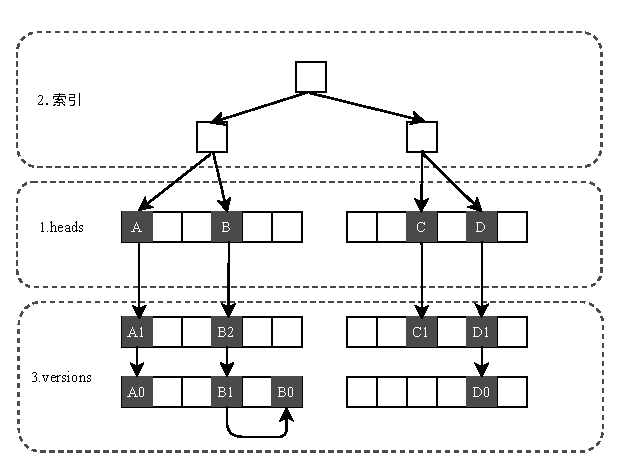
\includegraphics[width=1\linewidth]{recovery.pdf}
    \caption{记录数据的恢复步骤}
    \label{fig:record-recovery}
\end{figure}

首先是过滤所有不可见的以及未分配的 head。
一个数据库管理系统提供服务的前提是所有表格都有正确的索引来帮助事务查询,N2DB 也不例外。
N2DB 需要在所有可见的 head 上建立索引,因此需要将不可见的以及未分配的 head 过滤并回收掉。
表格的元数据中记录了 head pages,根据 head pages 中的地址,系统可以找到属于该表格的所有页面,进而找到了所有 head 的位置。
接下来系统需要扫描所有的 head,依次判断其是否是可回收的。
head 的可见性判断如图~\ref{fig:head-visibility} 所示。
head 首先需要判断最新版本是否为空,若为空则意味着该 head 是不可见的。
如果 head 对应的最新版本不为空,且最新版本是可见的,则意味着该 head 是可见的,因此该版本链是合法的。
版本可见性的判断与图~\ref{fig:version-visibility} 中相同。
最后如果 head 的最新版本是不可见的,但最新版本仍有较老的版本,那么该 head 也是可见的,版本链也是合法的。在此步骤中,由于 head 分配的无日志特性,系统只能通过扫描一个表格中所有的 head,依次判断每个 head 的可见性。同时系统在扫描的过程中会将所有不可见的版本回收,以防止内存泄漏问题。

\begin{figure}[ht]
    \centering
    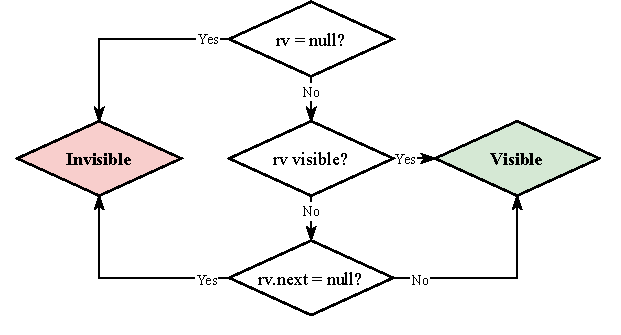
\includegraphics[width=1\linewidth]{figures/head_visibility.pdf}
    \caption{head 的可见性判断}
    \label{fig:head-visibility}
\end{figure}

第二是根据所有可见的 head 建立表格索引。
在扫描结束之后,系统将所有 head 对应的地址以及主键添加到新建的索引中。
版本链中此时仍存在不可见的版本,但是事务可以通过版本可见性无视版本链中中止事务以及中断事务所创建的不一致的 version。
因此当每个表格的索引重建之后,N2DB 就可以正常地相应请求了。

最后是回收所有未分配的 version。回收未分配的 version 是防止内存泄漏的关键。
由于 version 的分配也是无日志的,因此 version 分配与否当且仅当该 version 是否存在于一个合法的版本链中。
因此在索引建立之后,系统将会启动一个后台的扫描线程。
该线程负责扫描的版本链,并且记录版本链中所有 version 的位置信息。
该线程通过排除法可以得到所有未分配的 version 的位置信息,然后该线程会将未分配的 version 的信息传递给垃圾回收调度器。
后台扫描线程在扫描版本链的过程中,同样会识别出中止事务以及中断事务所创建的不可见的版本。
尽管这些版本不影响事务执行的正确性,但会影响事务的性能。因此后台扫描线程会将这些版本信息封装成 GCItem 传递给各个线程的垃圾回收调度器。

\section{数据恢复的正确性}

N2DB 中存在两个层面的数据管理。
一是 NVM 分配器采用页粒度管理和分配 NVM 空间。
二是 N2DB 中的表格在申请的页面上分配 head 以及 version。
因此 N2DB 需要保证两个层面的数据恢复工作都是正确的。

\subsection{NVM 分配器的数据恢复的正确性}

章节~\ref{ssec:nvm-alloc} 中定义了 NVM 分配器的可恢复性,即 NVM 分配器能否在重启之后将分配器的元数据中恢复到一个合法的状态。
合法的状态意味着对于 NVM 分配器而言,只有被使用的空间是已分配的,未被使用的空间均是未分配的,而且所有空间当且仅有一种状态。
一个空间被使用的判断标准在于该空间的地址是否被记录在 NVM 上。
根据 NVM 分配器的设计,一个页面在分配中,页面信息的记录一定晚于 bitmap 中分配信息的设置。
因此在系统重启之后,NVM 的页面当且仅有三种情况,未分配的,已分配且被使用的,以及分配但未被使用的。
前者可以通过章节~\ref{ssec:allocator-recovery} 中的步骤来回收,而第三种将由章节~\ref{ssec:metadata-recovery} 中的步骤来回收。
当两步回收均结束之后,NVM 分配器的元数据,也就是位图,会被设置成合法的状态。

\subsection{数据库的数据恢复的正确性}

数据库的数据恢复的正确在于能否保证提交事务的影响的持久化以及消除未提交事务的影响。

在元数据的恢复阶段中,N2DB 根据 NVM 分配器中的根指针,可以得到数据库中所有元数据的数据结构的地址信息。进而 N2DB 可以找到所有表格的记录相关数据结构的地址信息。

所有提交事务的影响包括 head 以及 version 的修改。由于系统保证在事务提交前事务的修改就已经持久化了,因此当 N2DB 找到所有版本链的入口时,提交事务的影响就没有丢失。未提交事务的影响同样也包括 head 以及 version 的修改。同时未提交事务包括两种,一种是中止事务,另一种是中断事务。

未提交事务对于 head 的影响是由 head 可见性来消除的。一个 head 是不可见的当且仅有三种情况:
\begin{enumerate}
    \item 该 head 是未分配的。一个 head 如果尚未被分配,那么该 head 的 newest\_version 应该为空指针。
    \item 该 head 是由一个中止事务或者中断事务插入的。根据章节~\ref{sec:mvcc} 中的插入流程,系统宕机可能发生在 head 修改 newest\_version 之前和之后。当宕机发生在 head 修改指针之前时,该 head 的 newest\_version 为空指针。当宕机发生在 head 修改指针之后时,该 head 的 newest\_version 所指向的版本应该是不合法的,其创建者也就是 xmin 对应的事务是未提交的。
    \item 该 head 已被删除,但尚未被垃圾回收。那么该 head 的 newest\_version 所对应的版本是被一个提交事务所废弃的。
\end{enumerate}
上述 head 的三种情况的分析可以看出 head 的可见性判断是完备的。
N2DB 根据 head 的可见性判断足以消除所有未提交事务对于 head 的影响。

未提交事务对于 version 的影响会被版本可见性判断无视掉。
一个未提交事务创建的版本当且仅有两种情况:
\begin{enumerate}
    \item 该 version 尚未被链接在版本链上。此类 version 会被后台的扫描线程视为未分配的,之后会被垃圾回收调度器回收。
    \item 该 version 已经被链接到版本链上,但事务未提交。version 的数据写入用于发生在其被链接在版本链上,因此 version 的 xmin 中的信息可以说明该版本是由一个未提交事务创建的。因此其他事务在运行时会无视掉此类版本。
\end{enumerate}
无论是哪一种情况,未提交事务相关的 version 都不会影响到后续事务的执行。

综上所述,N2DB 在数据恢复阶段结束后,提交事务的影响是持久化的。
而未提交事务的一部分影响被立刻消除。
另外一部分影响会被被其他事务无视,并且会被异步地消除。
因此 N2DB 的数据恢复机制是满足两个恢复原则的,其既可以保证事务的原子性也保证了事务的持久化。

\section{系统工程实现}
本章节将从代码级层面介绍数据恢复的机制的几个重要环节的系统工程实现。首先章节~\ref{ssec:data-structure-recovery} 会介绍 NVM 分配器的指针区域以及数据库的元数据的数据结构设计。
接下来章节~\ref{ssec:record-data-recovery} 会详细说明表格的记录数据恢复的流程。
最后章节~\ref{ssec:background-scan} 将简单提及后台扫描线程的流程。

\subsection{持久化指针的数据结构设计}
\label{ssec:data-structure-recovery}

为了保证系统能够在恢复时找到所有的数据结构,NVM 分配器中新增了持久化指针数组(PersistRootArray)这个数据结构。
持久化指针提供了访问指针以及持久化根指针的接口。
当系统第一次启动时会新建一个 N2DB 元数据,并且将根指针持久化到该数组第一个的位置。
持久化指针数组的数据结构定义如下:
\begin{itemize}
    \item 指针数量(root\_cnt):指针数量记录了存储于该数组的根指针的个数。
    \item 指针数组(roots):指针数组上记录了各个数据结构的根指针入口。
\end{itemize}



\subsection{元数据的数据结构设计}

数据库的所有元数据记录了存储引擎,数据库,表格以及列的所有元信息。
同时系统在创建数据库,表格等行为时,会修改不同类型的元数据。
为了保证数据结构的崩溃一致性,元数据的修改方法需要专门设计,以防止各个元数据之间数据的不一致。
本章节将依次介绍各个元数据的数据结构设计。

首先是 N2DB 的元数据。N2DB 的元数据主要记录着 N2DB 中数据库的数量以及各个数据库的元数据的指针。其具体的数据结构定义如下:
\begin{itemize}
    \item 初始化标志(is\_initialized):该标志表示该元数据是否被初始过。如果没有初始过则说明 N2DB 第一次启动。
    \item 数据库数量(database\_count):该变量记录了 N2DB 中数据库的数量。
    \item 数据库元数据入口(database\_entries):数据库元数据入口是一个数据库元数据指针的数组。
\end{itemize}

其次是数据库元数据。数据库元数据记录着数据库的标识符,名称等信息,同时存储着从属于该数据库的数量以及各个表格的元数据的指针。
具体的数据结构定义如下:
\begin{itemize}
    \item 初始化标志(is\_initialized):该标志用于判断该元数据是否被初始过。数据库在创建的过程中会先设置其他的成员变量的数据,最后原子化设置该标志,如果该标志不为 1,则数据库视为创建失败。
    \item 数据库标识符(database\_id):每个数据库都有全局唯一的数字标识符。
    \item 表格数量(table\_count):该变量记录了从属于数据库的表格的数量。
    \item 表格元数据入口(table\_entries):表格元数据入口是一个定长的数组,其中每一个元素均是表格元数据的指针。。
\end{itemize}

最后是表格元数据。
表格元数据记录着表格标识符,名称等基本信息。
表格元数据还记录着表格的模式信息,即每个列的类型,大小,名称等信息。
由于表格会在运行时申请页面,表格元数据中还需要记录表格申请的页面的地址。
表格元数据的数据结构定义如下:
\begin{itemize}
    \item 初始化标志(is\_initialized):该标志用于判断该元数据是否被初始过。
    \item 表格标识符(table\_id):每个表格的全局唯一的数字标识符。
    \item 列数(col\_count):列数记录了表格的列的数量。
    \item 列信息数组(col\_infos):列信息数组用于记录表格的模式信息。数组中每一个列信息均是一个三元组,分别记录了列名称,列大小以及列类型。
    \item head 页面入口(head\_pages\_entris):head 页面入口是一个数组,其中每一个元素均是一个页面指针。每个页面都是专门用来存放表格的 head。
    \item version 页面入口(version\_pages\_entries):version 页面入口同样也是一个页面指针数组。其中的每个页面都是专门用来存放表格的 version。
\end{itemize}


\begin{algorithm}[ht]
    \caption{使用表格名称创建一个新的表格, $create\_table\_with\_name$}
    \label{alg:create-table}
    \KwIn{The name of new table, $tbl\_name$ and schema}
    \KwOut{Success or not}
    \BlankLine
    Lock the database metadata;

    \If{ A table named $db\_name$ found}{
        Unlock the database metadata;

        return $false$;
    }

    NVM allocator a new page, $table\_data$;

    Get a new table id, $table\_id$;

    NVM allocator two new page for a new table;

    Modify $table\_data$ and persist;

    $table\_entries[table\_count] = table\_data$;

    Fence;

    $table\_count++$;

    Fence;

    Unlock the database metadata;

    return $true$;
\end{algorithm}

如前文所说,N2DB 中的数据库的创建,表格的创建会涉及多个元数据。
以创建表格为例,N2DB 在创建表格的过程会修改分配器的元数据,数据库的元数据以及表格的元数据。
如何正确设计几个元数据之间的持久化顺序是一大问题。
本文所实现的创建表格的具体流程展示在算法~\ref{alg:create-table} 中。
首先数据库元数据需要上锁,以防止别的线程并发访问该元数据。
接下来 NVM 分配器分配一个新的页面给表格元数据。
数据库元数据获取一个新的表格标识符。
NVM 分配器为表格多申请两个页面。表格需要这两个页面存放页面指针。
之后表格相关的元数据,比如表格标识符,名称,模式信息以及两个页面指针数组的地址都记录在 $table\_data$ 中。
之后系统更新数据库元数据,并且解锁该元数据。

通过该流程可以看出,如果系统在中间的步骤宕机了,会导致各个元数据之间的数据的不一致。
在数据恢复阶段,系统仅根据表格数量就来判断表格创建与否,而不根据其他信息。
根据创建表格这个例子可以看出,即使创建表格的过程中写的数据量远大于一个字节,系统仍可以通过一个字节的原子写来保证此过程的原子性。数据库中其他元数据的更新流程也是遵循此原则设计的。
不过该设计方法会在恢复时引入一些额外的开销。如果在数据恢复阶段系统发现了元数据之间的不一致,系统需要立刻对元数据进行修改。


\subsection{表格记录数据的恢复流程}
\label{ssec:record-data-recovery}

\begin{algorithm}[ht]
    \caption{表格重新加载 head 的流程,$reload\_head$}
    \label{alg:reload-heads}
    \BlankLine

    Calculate the length of head;

    Calculate the number of head in one page, $head\_per\_page$;

    Create a new index;

    \For{
        page $p$ in $head\_page\_entries[0:head\_page\_count]$
    }
    {
        \For{
            head $rh$ in $p[0:head\_per\_pages]$
        }{
            $rv = rh.newset\_version$;

            \eIf{$is\_recyable(rh)$}{
                Table reclaims $rh$;
            } {
                Insert $rh$ in the index;
            }

        }
    }
\end{algorithm}



N2DB 的过滤不可见的 head 流程如算法~\ref{alg:reload-heads} 所示。
系统根据元数据中的模式信息计算出一个 head 的长度以及一个页面上能够存放几个 head。
接下来系统创建一个新的索引。
系统根据 $head\_page\_entries$ 以及 $ head\_page\_count$ 两个数据得到该表格用于存储 head 的所有页面的地址。系统扫描每个页面上的所有的 head,依次判断各个 head 是否满足回收条件,并且回收可回收的 head。

\begin{algorithm}[ht]
    \caption{判断 head 是否可以回收,$is\_recyclable$}
    \label{alg:head-visibility}
    \KwIn{A head, $h$}
    \KwOut{Recyclable or not}
    \BlankLine

    $v = h.newest\_version$

    \If{$v == nullptr$}{
        return $true$;
    }


    \If{The transaction with $rv.xmax$ is COMMITTED} {
        return $true$;
    }

    \If{The transaction with $rv.xmin$ is ABORTED and $rv.prev\_version == nullptr$} {
        return $true$;
    }

    return $false$;


\end{algorithm}

算法~\ref{alg:head-visibility} 中展示了判断 head 是否可回收的具体过程。
首先查看该 head 的最新版本,若为空则该 head 可回收。
然后判断最新版本是否是提交事务删除的,如果是的话,则该 head 可回收。
最后判断最新版本的创建是否为中止的,并且没有更老的版本,如果满足该条件则该 head 也是可回收的。

\subsection{后台扫描线程的设计}
\label{ssec:background-scan}

后台扫描线程会依次回收每个表格的未分配的空间。后台线程扫描一个表格的版本链的过程如算法~\ref{alg:scan-versions} 中所示。扫描函数的输入分别是一个表格的可见的 head 的集合以及在系统重启时该表格的 $version\_page\_count$。$sacn\_version\_chain$ 函数首先创建两个数组,一个用于存储 version 的地址,一个用于存储扫描过程中遇到的不可见的 version。
接下来该线程将扫描所有的版本链,并且记录所有 version 的地址,如果该 version 是不可见的,将其封装成一个 GCItem。该线程会将一部分的 version 过滤掉。这部分 version 不属于该表格在数据恢复时的 $version\_page\_entries$ 的页面。线程将剩余的 version 排序,并且生成未分配的 version 的数组。
最后线程依次回收的 version,并且将扫描过程中遇到的不可见的 version 所对应的 GCItem 传递给垃圾回收调度器。


\begin{algorithm}[ht]
    \caption{数据恢复阶段的后台的扫描流程,$scan\_version\_chain$}
    \label{alg:scan-versions}
    \KwIn{Visible heads of a table, $heads$, $version\_page\_count$}
    \BlankLine

    Create a empty array of version, $versions$

    Create a empty array of GCItem, $gc\_list$

    \For{ head $h$ in $heads$}{
        \For{
            version $v$ in the version chain of $h$
        }{
            Insert $v$ into $versions$;

            \If{
                $v$ is invisible
            }{
                Pack $v$ as a GCItem and insert it into $gc\_list$;
            }
        }
    }

    Filter out $v$ that is not in $version\_page\_entries[0:version\_page_count]$;

    Sort $versions$ according to address;


    Generate unallocated versions $unallocated\_versions$ using $versions$;

    \For{version $v$ in $unallocated\_version$}{
        Table reclaims $v$;
    }

    \For{
        GCItem $item$ in $gc\_list$
    }{
        GCScheduler.schedule(item);
    }

\end{algorithm}

\section{本章小结}

本章节主要介绍了数据恢复机制的设计目标,设计思路以及正确性,其中还介绍了存储引擎的修改。同时为了详细介绍数据恢复的流程,本章节还从代码层面介绍了数据恢复机制中相关的三个重要的环节。

首先是数据恢复机制的设计目标。
虽然 NVM 的数据是持久化的,但是如果没有正确的元信息,NVM 上的数据将无法解读的字节流。
因此 N2DB 需要能够找到 NVM 上所有的数据结构。同时又因为 N2DB 需要保证事务的持久化以及原子性,数据恢复机制还对记录数据进行恢复。本文将设计目标总结为三点,分别是重构页面分配信息,恢复数据结构以及保证事务的原子性和持久化。

接着是存储引擎的修改。为了达成三个设计目标,N2DB 必须修改存储引擎的结构,尤其是 NVM 分配器和元数据的存储方式。NVM 分配器中添加一个持久化指针数组,其用于存储所有数据结构的根指针。
而存储引擎新增了元数据区,以树状结构来组织和管理各个层级的元数据。

然后是数据恢复机制的设计思路。
根据三个设计目标,本文将数据恢复流程大致分为三个阶段。
首先是 NVM 分配器的恢复。NVM 分配器是负责管理和分配 NVM 空间的。
因此 NVM 分配器的页面分配信息必须恢复到合法的状态,NVM 分配器还需要回收未分配及分配但未被使用的的页面。
接下来是元数据的恢复,本文将元数据组织成一个树状结构,并且在各个层级都存储了重要的元信息。
因此系统在数据恢复的过程中能够找到所有数据结构的位置。
系统同样需要根据元信息正确设置事务相关的状态,同时协助 NVM 分配器回收分配但未被使用的空间。最后则是记录数据的恢复,记录数据的恢复的目的在于遵循两个恢复原则,重新构造索引以及回收未分配的空间。记录数据恢复分为三步,过滤不可见的 head,重新构造索引以及使用后台扫描线程回收未分配的 version。系统重新构造索引后就能正常地提供服务。

之后是数据恢复机制的正确性。N2DB 的数据恢复的正确性可以分为两个层面。一层面是 NVM 分配器的数据恢复的正确性,这取决于在恢复后,NVM 分配器能否得到正确的分配信息。
另一部分是数据库的数据恢复的正确性,这取决于两点,一个保证提交事务的影响的持久化,二是消除未提交事务的影响。通过对每种情况分类讨论,本章节论证了 N2DB 数据恢复机制的正确性。

最后是数据恢复机制的系统实现。本章节首先介绍了持久化数组以及各个元数据的数据结构设计。
本章节进一步阐述了所有 NVM 数据结构修改的原则,即通过原子修改一个标志位来原子化一个复杂的数据结构修改。
接着本章节介绍了数据恢复过程中较为重要的记录数据恢复的流程,同时从代码层面解释 head 可见性的判断标准。
最后本章节介绍了后台扫描线程的主要工作流程。


